

\tikzset{every picture/.style={line width=0.75pt}} %set default line width to 0.75pt        

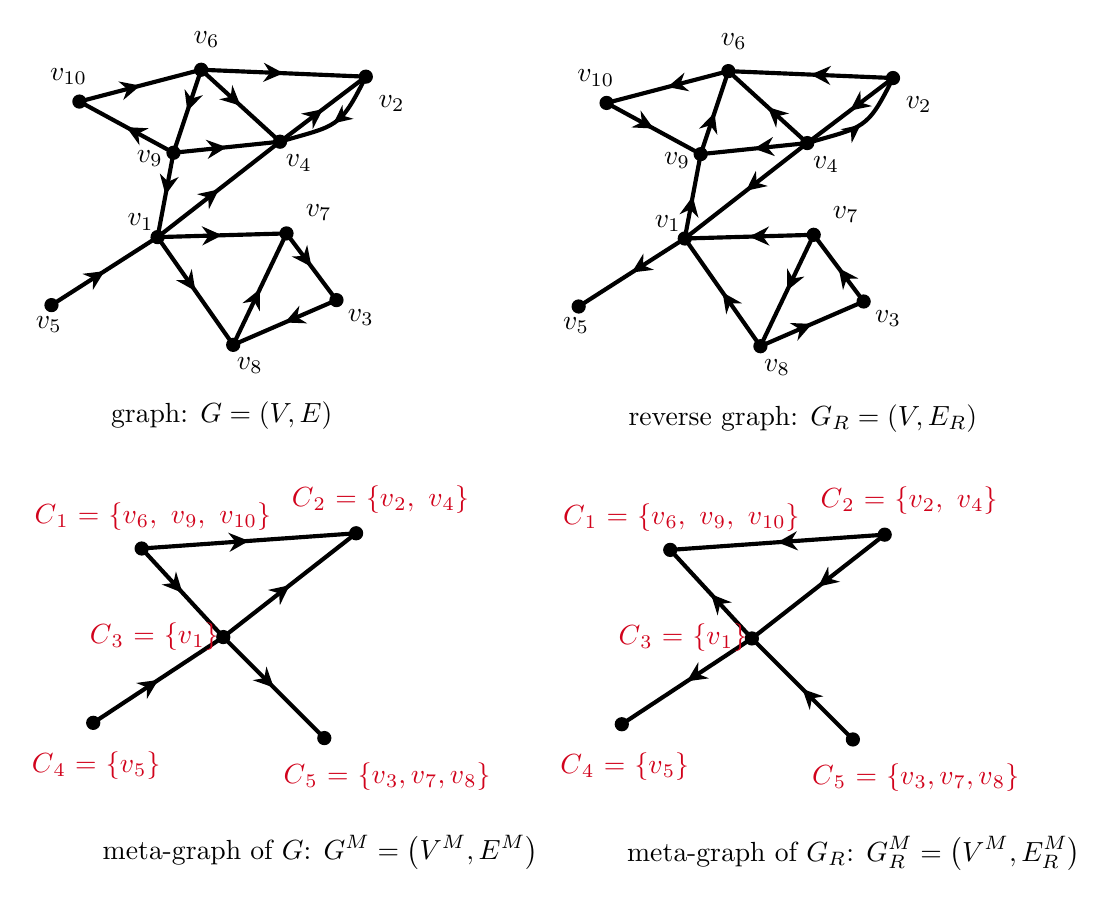
\begin{tikzpicture}[x=0.5pt,y=0.5pt,yscale=-1,xscale=1]
%uncomment if require: \path (0,615); %set diagram left start at 0, and has height of 615

%Flowchart: Connector [id:dp35531003904401826] 
\draw  [fill={rgb, 255:red, 0; green, 0; blue, 0 }  ,fill opacity=1 ] (87,378) .. controls (87,375.58) and (88.96,373.62) .. (91.38,373.62) .. controls (93.79,373.62) and (95.75,375.58) .. (95.75,378) .. controls (95.75,380.42) and (93.79,382.38) .. (91.38,382.38) .. controls (88.96,382.38) and (87,380.42) .. (87,378) -- cycle ;
%Straight Lines [id:da06413387293276729] 
\draw [color={rgb, 255:red, 0; green, 0; blue, 0 }  ,draw opacity=1 ][line width=1.5]    (114.38,92) -- (134.38,32) ;
\draw [shift={(124.38,62)}, rotate = 288.43] [fill={rgb, 255:red, 0; green, 0; blue, 0 }  ,fill opacity=1 ][line width=0.08]  [draw opacity=0] (14.56,-6.99) -- (0,0) -- (14.56,6.99) -- (9.67,0) -- cycle    ;
%Straight Lines [id:da9572573982067856] 
\draw [color={rgb, 255:red, 0; green, 0; blue, 0 }  ,draw opacity=1 ][line width=1.5]    (134.38,32) -- (46.38,55) ;
\draw [shift={(90.38,43.5)}, rotate = 165.35] [fill={rgb, 255:red, 0; green, 0; blue, 0 }  ,fill opacity=1 ][line width=0.08]  [draw opacity=0] (14.56,-6.99) -- (0,0) -- (14.56,6.99) -- (9.67,0) -- cycle    ;
%Straight Lines [id:da027017237295007268] 
\draw [color={rgb, 255:red, 0; green, 0; blue, 0 }  ,draw opacity=1 ][line width=1.5]    (150.38,442) -- (91.38,378) ;
\draw [shift={(120.88,410)}, rotate = 227.33] [fill={rgb, 255:red, 0; green, 0; blue, 0 }  ,fill opacity=1 ][line width=0.08]  [draw opacity=0] (14.56,-6.99) -- (0,0) -- (14.56,6.99) -- (9.67,0) -- cycle    ;
%Flowchart: Connector [id:dp7018202329285442] 
\draw  [fill={rgb, 255:red, 0; green, 0; blue, 0 }  ,fill opacity=1 ] (242,367) .. controls (242,364.58) and (243.96,362.62) .. (246.38,362.62) .. controls (248.79,362.62) and (250.75,364.58) .. (250.75,367) .. controls (250.75,369.42) and (248.79,371.38) .. (246.38,371.38) .. controls (243.96,371.38) and (242,369.42) .. (242,367) -- cycle ;
%Flowchart: Connector [id:dp9468304553677146] 
\draw  [fill={rgb, 255:red, 0; green, 0; blue, 0 }  ,fill opacity=1 ] (249,37) .. controls (249,34.58) and (250.96,32.62) .. (253.38,32.62) .. controls (255.79,32.62) and (257.75,34.58) .. (257.75,37) .. controls (257.75,39.42) and (255.79,41.38) .. (253.38,41.38) .. controls (250.96,41.38) and (249,39.42) .. (249,37) -- cycle ;
%Flowchart: Connector [id:dp10084257988995149] 
\draw  [fill={rgb, 255:red, 0; green, 0; blue, 0 }  ,fill opacity=1 ] (187,84) .. controls (187,81.58) and (188.96,79.62) .. (191.38,79.62) .. controls (193.79,79.62) and (195.75,81.58) .. (195.75,84) .. controls (195.75,86.42) and (193.79,88.38) .. (191.38,88.38) .. controls (188.96,88.38) and (187,86.42) .. (187,84) -- cycle ;
%Flowchart: Connector [id:dp5678652918378437] 
\draw  [fill={rgb, 255:red, 0; green, 0; blue, 0 }  ,fill opacity=1 ] (191.99,148.72) .. controls (192.85,146.46) and (195.39,145.34) .. (197.64,146.21) .. controls (199.9,147.08) and (201.02,149.61) .. (200.15,151.86) .. controls (199.28,154.12) and (196.75,155.24) .. (194.5,154.38) .. controls (192.24,153.51) and (191.12,150.97) .. (191.99,148.72) -- cycle ;
%Flowchart: Connector [id:dp9451957343710085] 
\draw  [fill={rgb, 255:red, 0; green, 0; blue, 0 }  ,fill opacity=1 ] (228.07,196.91) .. controls (228.94,194.66) and (231.47,193.53) .. (233.73,194.4) .. controls (235.98,195.27) and (237.11,197.8) .. (236.24,200.06) .. controls (235.37,202.32) and (232.84,203.44) .. (230.58,202.57) .. controls (228.33,201.7) and (227.2,199.17) .. (228.07,196.91) -- cycle ;
%Flowchart: Connector [id:dp7598246465914121] 
\draw  [fill={rgb, 255:red, 0; green, 0; blue, 0 }  ,fill opacity=1 ] (153.46,229.25) .. controls (154.33,227) and (156.86,225.87) .. (159.11,226.74) .. controls (161.37,227.61) and (162.49,230.14) .. (161.63,232.4) .. controls (160.76,234.65) and (158.22,235.78) .. (155.97,234.91) .. controls (153.71,234.04) and (152.59,231.51) .. (153.46,229.25) -- cycle ;
%Flowchart: Connector [id:dp9270593548114698] 
\draw  [fill={rgb, 255:red, 0; green, 0; blue, 0 }  ,fill opacity=1 ] (22.12,200.53) .. controls (22.99,198.28) and (25.52,197.15) .. (27.77,198.02) .. controls (30.03,198.89) and (31.15,201.42) .. (30.28,203.68) .. controls (29.42,205.94) and (26.88,207.06) .. (24.63,206.19) .. controls (22.37,205.32) and (21.25,202.79) .. (22.12,200.53) -- cycle ;
%Flowchart: Connector [id:dp0003313036349563703] 
\draw  [fill={rgb, 255:red, 0; green, 0; blue, 0 }  ,fill opacity=1 ] (98.79,151.39) .. controls (99.66,149.14) and (102.2,148.01) .. (104.45,148.88) .. controls (106.71,149.75) and (107.83,152.28) .. (106.96,154.54) .. controls (106.09,156.8) and (103.56,157.92) .. (101.3,157.05) .. controls (99.05,156.18) and (97.92,153.65) .. (98.79,151.39) -- cycle ;
%Flowchart: Connector [id:dp05524410597346219] 
\draw  [fill={rgb, 255:red, 0; green, 0; blue, 0 }  ,fill opacity=1 ] (130,32) .. controls (130,29.58) and (131.96,27.62) .. (134.38,27.62) .. controls (136.79,27.62) and (138.75,29.58) .. (138.75,32) .. controls (138.75,34.42) and (136.79,36.38) .. (134.38,36.38) .. controls (131.96,36.38) and (130,34.42) .. (130,32) -- cycle ;
%Flowchart: Connector [id:dp8722833316705884] 
\draw  [fill={rgb, 255:red, 0; green, 0; blue, 0 }  ,fill opacity=1 ] (42,55) .. controls (42,52.58) and (43.96,50.62) .. (46.38,50.62) .. controls (48.79,50.62) and (50.75,52.58) .. (50.75,55) .. controls (50.75,57.42) and (48.79,59.38) .. (46.38,59.38) .. controls (43.96,59.38) and (42,57.42) .. (42,55) -- cycle ;
%Flowchart: Connector [id:dp04902898021909796] 
\draw  [fill={rgb, 255:red, 0; green, 0; blue, 0 }  ,fill opacity=1 ] (110,92) .. controls (110,89.58) and (111.96,87.62) .. (114.38,87.62) .. controls (116.79,87.62) and (118.75,89.58) .. (118.75,92) .. controls (118.75,94.42) and (116.79,96.38) .. (114.38,96.38) .. controls (111.96,96.38) and (110,94.42) .. (110,92) -- cycle ;
%Straight Lines [id:da6957258198444844] 
\draw [color={rgb, 255:red, 0; green, 0; blue, 0 }  ,draw opacity=1 ][line width=1.5]    (46.38,55) -- (114.38,92) ;
\draw [shift={(80.38,73.5)}, rotate = 28.55] [fill={rgb, 255:red, 0; green, 0; blue, 0 }  ,fill opacity=1 ][line width=0.08]  [draw opacity=0] (14.56,-6.99) -- (0,0) -- (14.56,6.99) -- (9.67,0) -- cycle    ;
%Straight Lines [id:da1865955612168957] 
\draw [color={rgb, 255:red, 0; green, 0; blue, 0 }  ,draw opacity=1 ][line width=1.5]    (102.88,152.97) -- (114.38,92) ;
\draw [shift={(108.63,122.48)}, rotate = 280.68] [fill={rgb, 255:red, 0; green, 0; blue, 0 }  ,fill opacity=1 ][line width=0.08]  [draw opacity=0] (14.56,-6.99) -- (0,0) -- (14.56,6.99) -- (9.67,0) -- cycle    ;
%Straight Lines [id:da5983156386140572] 
\draw [color={rgb, 255:red, 0; green, 0; blue, 0 }  ,draw opacity=1 ][line width=1.5]    (102.88,152.97) -- (26.2,202.11) ;
\draw [shift={(64.54,177.54)}, rotate = 147.35] [fill={rgb, 255:red, 0; green, 0; blue, 0 }  ,fill opacity=1 ][line width=0.08]  [draw opacity=0] (14.56,-6.99) -- (0,0) -- (14.56,6.99) -- (9.67,0) -- cycle    ;
%Straight Lines [id:da7813440675788919] 
\draw [color={rgb, 255:red, 0; green, 0; blue, 0 }  ,draw opacity=1 ][line width=1.5]    (157.54,230.82) -- (102.88,152.97) ;
\draw [shift={(130.21,191.9)}, rotate = 234.93] [fill={rgb, 255:red, 0; green, 0; blue, 0 }  ,fill opacity=1 ][line width=0.08]  [draw opacity=0] (14.56,-6.99) -- (0,0) -- (14.56,6.99) -- (9.67,0) -- cycle    ;
%Straight Lines [id:da11231036470839317] 
\draw [color={rgb, 255:red, 0; green, 0; blue, 0 }  ,draw opacity=1 ][line width=1.5]    (196.07,150.29) -- (102.88,152.97) ;
\draw [shift={(149.47,151.63)}, rotate = 178.36] [fill={rgb, 255:red, 0; green, 0; blue, 0 }  ,fill opacity=1 ][line width=0.08]  [draw opacity=0] (14.56,-6.99) -- (0,0) -- (14.56,6.99) -- (9.67,0) -- cycle    ;
%Straight Lines [id:da3818914730957623] 
\draw [color={rgb, 255:red, 0; green, 0; blue, 0 }  ,draw opacity=1 ][line width=1.5]    (196.07,150.29) -- (157.54,230.82) ;
\draw [shift={(176.81,190.56)}, rotate = 115.57] [fill={rgb, 255:red, 0; green, 0; blue, 0 }  ,fill opacity=1 ][line width=0.08]  [draw opacity=0] (14.56,-6.99) -- (0,0) -- (14.56,6.99) -- (9.67,0) -- cycle    ;
%Straight Lines [id:da5617379482893489] 
\draw [color={rgb, 255:red, 0; green, 0; blue, 0 }  ,draw opacity=1 ][line width=1.5]    (157.54,230.82) -- (232.16,198.49) ;
\draw [shift={(194.85,214.66)}, rotate = 336.57] [fill={rgb, 255:red, 0; green, 0; blue, 0 }  ,fill opacity=1 ][line width=0.08]  [draw opacity=0] (14.56,-6.99) -- (0,0) -- (14.56,6.99) -- (9.67,0) -- cycle    ;
%Straight Lines [id:da7816864329937088] 
\draw [color={rgb, 255:red, 0; green, 0; blue, 0 }  ,draw opacity=1 ][line width=1.5]    (232.16,198.49) -- (196.07,150.29) ;
\draw [shift={(214.11,174.39)}, rotate = 233.18] [fill={rgb, 255:red, 0; green, 0; blue, 0 }  ,fill opacity=1 ][line width=0.08]  [draw opacity=0] (14.56,-6.99) -- (0,0) -- (14.56,6.99) -- (9.67,0) -- cycle    ;
%Straight Lines [id:da007998244336271831] 
\draw [color={rgb, 255:red, 0; green, 0; blue, 0 }  ,draw opacity=1 ][line width=1.5]    (191.38,84) -- (102.88,152.97) ;
\draw [shift={(147.13,118.48)}, rotate = 142.07] [fill={rgb, 255:red, 0; green, 0; blue, 0 }  ,fill opacity=1 ][line width=0.08]  [draw opacity=0] (14.56,-6.99) -- (0,0) -- (14.56,6.99) -- (9.67,0) -- cycle    ;
%Straight Lines [id:da07370415553910226] 
\draw [color={rgb, 255:red, 0; green, 0; blue, 0 }  ,draw opacity=1 ][line width=1.5]    (253.38,37) -- (191.38,84) ;
\draw [shift={(222.38,60.5)}, rotate = 142.84] [fill={rgb, 255:red, 0; green, 0; blue, 0 }  ,fill opacity=1 ][line width=0.08]  [draw opacity=0] (14.56,-6.99) -- (0,0) -- (14.56,6.99) -- (9.67,0) -- cycle    ;
%Straight Lines [id:da31265226854681183] 
\draw [color={rgb, 255:red, 0; green, 0; blue, 0 }  ,draw opacity=1 ][line width=1.5]    (253.38,37) -- (134.38,32) ;
\draw [shift={(193.88,34.5)}, rotate = 182.41] [fill={rgb, 255:red, 0; green, 0; blue, 0 }  ,fill opacity=1 ][line width=0.08]  [draw opacity=0] (14.56,-6.99) -- (0,0) -- (14.56,6.99) -- (9.67,0) -- cycle    ;
%Straight Lines [id:da03944598876714689] 
\draw [color={rgb, 255:red, 0; green, 0; blue, 0 }  ,draw opacity=1 ][line width=1.5]    (191.38,84) -- (114.38,92) ;
\draw [shift={(152.88,88)}, rotate = 174.07] [fill={rgb, 255:red, 0; green, 0; blue, 0 }  ,fill opacity=1 ][line width=0.08]  [draw opacity=0] (14.56,-6.99) -- (0,0) -- (14.56,6.99) -- (9.67,0) -- cycle    ;
%Curve Lines [id:da24538681443295773] 
\draw [line width=1.5]    (253.38,37) .. controls (234.5,75) and (232.5,72) .. (191.38,84) ;
\draw [shift={(229.99,70.74)}, rotate = 321.64] [fill={rgb, 255:red, 0; green, 0; blue, 0 }  ][line width=0.08]  [draw opacity=0] (13.4,-6.43) -- (0,0) -- (13.4,6.44) -- (8.9,0) -- cycle    ;
%Straight Lines [id:da5495061302418803] 
\draw [color={rgb, 255:red, 0; green, 0; blue, 0 }  ,draw opacity=1 ][line width=1.5]    (191.38,84) -- (134.38,32) ;
\draw [shift={(162.88,58)}, rotate = 222.37] [fill={rgb, 255:red, 0; green, 0; blue, 0 }  ,fill opacity=1 ][line width=0.08]  [draw opacity=0] (14.56,-6.99) -- (0,0) -- (14.56,6.99) -- (9.67,0) -- cycle    ;
%Flowchart: Connector [id:dp24932583909944328] 
\draw  [fill={rgb, 255:red, 0; green, 0; blue, 0 }  ,fill opacity=1 ] (146,442) .. controls (146,439.58) and (147.96,437.62) .. (150.38,437.62) .. controls (152.79,437.62) and (154.75,439.58) .. (154.75,442) .. controls (154.75,444.42) and (152.79,446.38) .. (150.38,446.38) .. controls (147.96,446.38) and (146,444.42) .. (146,442) -- cycle ;
%Flowchart: Connector [id:dp3666265572902413] 
\draw  [fill={rgb, 255:red, 0; green, 0; blue, 0 }  ,fill opacity=1 ] (52,504) .. controls (52,501.58) and (53.96,499.62) .. (56.38,499.62) .. controls (58.79,499.62) and (60.75,501.58) .. (60.75,504) .. controls (60.75,506.42) and (58.79,508.38) .. (56.38,508.38) .. controls (53.96,508.38) and (52,506.42) .. (52,504) -- cycle ;
%Flowchart: Connector [id:dp5809100494545972] 
\draw  [fill={rgb, 255:red, 0; green, 0; blue, 0 }  ,fill opacity=1 ] (219,515) .. controls (219,512.58) and (220.96,510.62) .. (223.38,510.62) .. controls (225.79,510.62) and (227.75,512.58) .. (227.75,515) .. controls (227.75,517.42) and (225.79,519.38) .. (223.38,519.38) .. controls (220.96,519.38) and (219,517.42) .. (219,515) -- cycle ;
%Straight Lines [id:da1229562998864333] 
\draw [color={rgb, 255:red, 0; green, 0; blue, 0 }  ,draw opacity=1 ][line width=1.5]    (246.38,367) -- (91.38,378) ;
\draw [shift={(168.88,372.5)}, rotate = 175.94] [fill={rgb, 255:red, 0; green, 0; blue, 0 }  ,fill opacity=1 ][line width=0.08]  [draw opacity=0] (14.56,-6.99) -- (0,0) -- (14.56,6.99) -- (9.67,0) -- cycle    ;
%Straight Lines [id:da6177657045500177] 
\draw [color={rgb, 255:red, 0; green, 0; blue, 0 }  ,draw opacity=1 ][line width=1.5]    (246.38,367) -- (150.38,442) ;
\draw [shift={(198.38,404.5)}, rotate = 142] [fill={rgb, 255:red, 0; green, 0; blue, 0 }  ,fill opacity=1 ][line width=0.08]  [draw opacity=0] (14.56,-6.99) -- (0,0) -- (14.56,6.99) -- (9.67,0) -- cycle    ;
%Straight Lines [id:da45439161896636415] 
\draw [color={rgb, 255:red, 0; green, 0; blue, 0 }  ,draw opacity=1 ][line width=1.5]    (223.38,515) -- (150.38,442) ;
\draw [shift={(186.88,478.5)}, rotate = 225] [fill={rgb, 255:red, 0; green, 0; blue, 0 }  ,fill opacity=1 ][line width=0.08]  [draw opacity=0] (14.56,-6.99) -- (0,0) -- (14.56,6.99) -- (9.67,0) -- cycle    ;
%Straight Lines [id:da11561285868658588] 
\draw [color={rgb, 255:red, 0; green, 0; blue, 0 }  ,draw opacity=1 ][line width=1.5]    (150.38,442) -- (56.38,504) ;
\draw [shift={(103.38,473)}, rotate = 146.59] [fill={rgb, 255:red, 0; green, 0; blue, 0 }  ,fill opacity=1 ][line width=0.08]  [draw opacity=0] (14.56,-6.99) -- (0,0) -- (14.56,6.99) -- (9.67,0) -- cycle    ;
%Straight Lines [id:da8168779159006088] 
\draw [color={rgb, 255:red, 0; green, 0; blue, 0 }  ,draw opacity=1 ][line width=1.5]    (495.38,93) -- (515.38,33) ;
\draw [shift={(505.38,63)}, rotate = 468.43] [fill={rgb, 255:red, 0; green, 0; blue, 0 }  ,fill opacity=1 ][line width=0.08]  [draw opacity=0] (14.56,-6.99) -- (0,0) -- (14.56,6.99) -- (9.67,0) -- cycle    ;
%Straight Lines [id:da894325464874] 
\draw [color={rgb, 255:red, 0; green, 0; blue, 0 }  ,draw opacity=1 ][line width=1.5]    (515.38,33) -- (427.38,56) ;
\draw [shift={(471.38,44.5)}, rotate = 345.35] [fill={rgb, 255:red, 0; green, 0; blue, 0 }  ,fill opacity=1 ][line width=0.08]  [draw opacity=0] (14.56,-6.99) -- (0,0) -- (14.56,6.99) -- (9.67,0) -- cycle    ;
%Flowchart: Connector [id:dp2028061961127232] 
\draw  [fill={rgb, 255:red, 0; green, 0; blue, 0 }  ,fill opacity=1 ] (630,38) .. controls (630,35.58) and (631.96,33.62) .. (634.38,33.62) .. controls (636.79,33.62) and (638.75,35.58) .. (638.75,38) .. controls (638.75,40.42) and (636.79,42.38) .. (634.38,42.38) .. controls (631.96,42.38) and (630,40.42) .. (630,38) -- cycle ;
%Flowchart: Connector [id:dp6685886791876837] 
\draw  [fill={rgb, 255:red, 0; green, 0; blue, 0 }  ,fill opacity=1 ] (568,85) .. controls (568,82.58) and (569.96,80.62) .. (572.38,80.62) .. controls (574.79,80.62) and (576.75,82.58) .. (576.75,85) .. controls (576.75,87.42) and (574.79,89.38) .. (572.38,89.38) .. controls (569.96,89.38) and (568,87.42) .. (568,85) -- cycle ;
%Flowchart: Connector [id:dp6828969280331417] 
\draw  [fill={rgb, 255:red, 0; green, 0; blue, 0 }  ,fill opacity=1 ] (572.99,149.72) .. controls (573.85,147.46) and (576.39,146.34) .. (578.64,147.21) .. controls (580.9,148.08) and (582.02,150.61) .. (581.15,152.86) .. controls (580.28,155.12) and (577.75,156.24) .. (575.5,155.38) .. controls (573.24,154.51) and (572.12,151.97) .. (572.99,149.72) -- cycle ;
%Flowchart: Connector [id:dp5869007902050025] 
\draw  [fill={rgb, 255:red, 0; green, 0; blue, 0 }  ,fill opacity=1 ] (609.07,197.91) .. controls (609.94,195.66) and (612.47,194.53) .. (614.73,195.4) .. controls (616.98,196.27) and (618.11,198.8) .. (617.24,201.06) .. controls (616.37,203.32) and (613.84,204.44) .. (611.58,203.57) .. controls (609.33,202.7) and (608.2,200.17) .. (609.07,197.91) -- cycle ;
%Flowchart: Connector [id:dp29745484225367824] 
\draw  [fill={rgb, 255:red, 0; green, 0; blue, 0 }  ,fill opacity=1 ] (534.46,230.25) .. controls (535.33,228) and (537.86,226.87) .. (540.11,227.74) .. controls (542.37,228.61) and (543.49,231.14) .. (542.63,233.4) .. controls (541.76,235.65) and (539.22,236.78) .. (536.97,235.91) .. controls (534.71,235.04) and (533.59,232.51) .. (534.46,230.25) -- cycle ;
%Flowchart: Connector [id:dp9007070710643801] 
\draw  [fill={rgb, 255:red, 0; green, 0; blue, 0 }  ,fill opacity=1 ] (403.12,201.53) .. controls (403.99,199.28) and (406.52,198.15) .. (408.77,199.02) .. controls (411.03,199.89) and (412.15,202.42) .. (411.28,204.68) .. controls (410.42,206.94) and (407.88,208.06) .. (405.63,207.19) .. controls (403.37,206.32) and (402.25,203.79) .. (403.12,201.53) -- cycle ;
%Flowchart: Connector [id:dp8032522319169138] 
\draw  [fill={rgb, 255:red, 0; green, 0; blue, 0 }  ,fill opacity=1 ] (479.79,152.39) .. controls (480.66,150.14) and (483.2,149.01) .. (485.45,149.88) .. controls (487.71,150.75) and (488.83,153.28) .. (487.96,155.54) .. controls (487.09,157.8) and (484.56,158.92) .. (482.3,158.05) .. controls (480.05,157.18) and (478.92,154.65) .. (479.79,152.39) -- cycle ;
%Flowchart: Connector [id:dp3269943450949304] 
\draw  [fill={rgb, 255:red, 0; green, 0; blue, 0 }  ,fill opacity=1 ] (511,33) .. controls (511,30.58) and (512.96,28.62) .. (515.38,28.62) .. controls (517.79,28.62) and (519.75,30.58) .. (519.75,33) .. controls (519.75,35.42) and (517.79,37.38) .. (515.38,37.38) .. controls (512.96,37.38) and (511,35.42) .. (511,33) -- cycle ;
%Flowchart: Connector [id:dp23422253916024505] 
\draw  [fill={rgb, 255:red, 0; green, 0; blue, 0 }  ,fill opacity=1 ] (423,56) .. controls (423,53.58) and (424.96,51.62) .. (427.38,51.62) .. controls (429.79,51.62) and (431.75,53.58) .. (431.75,56) .. controls (431.75,58.42) and (429.79,60.38) .. (427.38,60.38) .. controls (424.96,60.38) and (423,58.42) .. (423,56) -- cycle ;
%Flowchart: Connector [id:dp010586655389437372] 
\draw  [fill={rgb, 255:red, 0; green, 0; blue, 0 }  ,fill opacity=1 ] (491,93) .. controls (491,90.58) and (492.96,88.62) .. (495.38,88.62) .. controls (497.79,88.62) and (499.75,90.58) .. (499.75,93) .. controls (499.75,95.42) and (497.79,97.38) .. (495.38,97.38) .. controls (492.96,97.38) and (491,95.42) .. (491,93) -- cycle ;
%Straight Lines [id:da51057635409129] 
\draw [color={rgb, 255:red, 0; green, 0; blue, 0 }  ,draw opacity=1 ][line width=1.5]    (427.38,56) -- (495.38,93) ;
\draw [shift={(461.38,74.5)}, rotate = 208.55] [fill={rgb, 255:red, 0; green, 0; blue, 0 }  ,fill opacity=1 ][line width=0.08]  [draw opacity=0] (14.56,-6.99) -- (0,0) -- (14.56,6.99) -- (9.67,0) -- cycle    ;
%Straight Lines [id:da9705884712552635] 
\draw [color={rgb, 255:red, 0; green, 0; blue, 0 }  ,draw opacity=1 ][line width=1.5]    (483.88,153.97) -- (495.38,93) ;
\draw [shift={(489.63,123.48)}, rotate = 460.68] [fill={rgb, 255:red, 0; green, 0; blue, 0 }  ,fill opacity=1 ][line width=0.08]  [draw opacity=0] (14.56,-6.99) -- (0,0) -- (14.56,6.99) -- (9.67,0) -- cycle    ;
%Straight Lines [id:da5127893862513866] 
\draw [color={rgb, 255:red, 0; green, 0; blue, 0 }  ,draw opacity=1 ][line width=1.5]    (483.88,153.97) -- (407.2,203.11) ;
\draw [shift={(445.54,178.54)}, rotate = 327.35] [fill={rgb, 255:red, 0; green, 0; blue, 0 }  ,fill opacity=1 ][line width=0.08]  [draw opacity=0] (14.56,-6.99) -- (0,0) -- (14.56,6.99) -- (9.67,0) -- cycle    ;
%Straight Lines [id:da5716196586001995] 
\draw [color={rgb, 255:red, 0; green, 0; blue, 0 }  ,draw opacity=1 ][line width=1.5]    (538.54,231.82) -- (483.88,153.97) ;
\draw [shift={(511.21,192.9)}, rotate = 414.93] [fill={rgb, 255:red, 0; green, 0; blue, 0 }  ,fill opacity=1 ][line width=0.08]  [draw opacity=0] (14.56,-6.99) -- (0,0) -- (14.56,6.99) -- (9.67,0) -- cycle    ;
%Straight Lines [id:da9185935928544606] 
\draw [color={rgb, 255:red, 0; green, 0; blue, 0 }  ,draw opacity=1 ][line width=1.5]    (577.07,151.29) -- (483.88,153.97) ;
\draw [shift={(530.47,152.63)}, rotate = 358.36] [fill={rgb, 255:red, 0; green, 0; blue, 0 }  ,fill opacity=1 ][line width=0.08]  [draw opacity=0] (14.56,-6.99) -- (0,0) -- (14.56,6.99) -- (9.67,0) -- cycle    ;
%Straight Lines [id:da5526780501990177] 
\draw [color={rgb, 255:red, 0; green, 0; blue, 0 }  ,draw opacity=1 ][line width=1.5]    (577.07,151.29) -- (538.54,231.82) ;
\draw [shift={(557.81,191.56)}, rotate = 295.57] [fill={rgb, 255:red, 0; green, 0; blue, 0 }  ,fill opacity=1 ][line width=0.08]  [draw opacity=0] (14.56,-6.99) -- (0,0) -- (14.56,6.99) -- (9.67,0) -- cycle    ;
%Straight Lines [id:da07669648878710078] 
\draw [color={rgb, 255:red, 0; green, 0; blue, 0 }  ,draw opacity=1 ][line width=1.5]    (538.54,231.82) -- (613.16,199.49) ;
\draw [shift={(575.85,215.66)}, rotate = 516.5699999999999] [fill={rgb, 255:red, 0; green, 0; blue, 0 }  ,fill opacity=1 ][line width=0.08]  [draw opacity=0] (14.56,-6.99) -- (0,0) -- (14.56,6.99) -- (9.67,0) -- cycle    ;
%Straight Lines [id:da04407384927929969] 
\draw [color={rgb, 255:red, 0; green, 0; blue, 0 }  ,draw opacity=1 ][line width=1.5]    (613.16,199.49) -- (577.07,151.29) ;
\draw [shift={(595.11,175.39)}, rotate = 413.18] [fill={rgb, 255:red, 0; green, 0; blue, 0 }  ,fill opacity=1 ][line width=0.08]  [draw opacity=0] (14.56,-6.99) -- (0,0) -- (14.56,6.99) -- (9.67,0) -- cycle    ;
%Straight Lines [id:da7736173583087967] 
\draw [color={rgb, 255:red, 0; green, 0; blue, 0 }  ,draw opacity=1 ][line width=1.5]    (572.38,85) -- (483.88,153.97) ;
\draw [shift={(528.13,119.48)}, rotate = 322.07] [fill={rgb, 255:red, 0; green, 0; blue, 0 }  ,fill opacity=1 ][line width=0.08]  [draw opacity=0] (14.56,-6.99) -- (0,0) -- (14.56,6.99) -- (9.67,0) -- cycle    ;
%Straight Lines [id:da984046162104014] 
\draw [color={rgb, 255:red, 0; green, 0; blue, 0 }  ,draw opacity=1 ][line width=1.5]    (634.38,38) -- (572.38,85) ;
\draw [shift={(603.38,61.5)}, rotate = 322.84000000000003] [fill={rgb, 255:red, 0; green, 0; blue, 0 }  ,fill opacity=1 ][line width=0.08]  [draw opacity=0] (14.56,-6.99) -- (0,0) -- (14.56,6.99) -- (9.67,0) -- cycle    ;
%Straight Lines [id:da41303131230822765] 
\draw [color={rgb, 255:red, 0; green, 0; blue, 0 }  ,draw opacity=1 ][line width=1.5]    (634.38,38) -- (515.38,33) ;
\draw [shift={(574.88,35.5)}, rotate = 362.40999999999997] [fill={rgb, 255:red, 0; green, 0; blue, 0 }  ,fill opacity=1 ][line width=0.08]  [draw opacity=0] (14.56,-6.99) -- (0,0) -- (14.56,6.99) -- (9.67,0) -- cycle    ;
%Straight Lines [id:da9312483814272712] 
\draw [color={rgb, 255:red, 0; green, 0; blue, 0 }  ,draw opacity=1 ][line width=1.5]    (572.38,85) -- (495.38,93) ;
\draw [shift={(533.88,89)}, rotate = 354.07] [fill={rgb, 255:red, 0; green, 0; blue, 0 }  ,fill opacity=1 ][line width=0.08]  [draw opacity=0] (14.56,-6.99) -- (0,0) -- (14.56,6.99) -- (9.67,0) -- cycle    ;
%Curve Lines [id:da6657670157747444] 
\draw [line width=1.5]    (634.38,38) .. controls (615.5,76) and (613.5,73) .. (572.38,85) ;
\draw [shift={(610.99,71.74)}, rotate = 141.64] [fill={rgb, 255:red, 0; green, 0; blue, 0 }  ][line width=0.08]  [draw opacity=0] (13.4,-6.43) -- (0,0) -- (13.4,6.44) -- (8.9,0) -- cycle    ;
%Straight Lines [id:da6019953764665212] 
\draw [color={rgb, 255:red, 0; green, 0; blue, 0 }  ,draw opacity=1 ][line width=1.5]    (572.38,85) -- (515.38,33) ;
\draw [shift={(543.88,59)}, rotate = 402.37] [fill={rgb, 255:red, 0; green, 0; blue, 0 }  ,fill opacity=1 ][line width=0.08]  [draw opacity=0] (14.56,-6.99) -- (0,0) -- (14.56,6.99) -- (9.67,0) -- cycle    ;
%Flowchart: Connector [id:dp2447453141676298] 
\draw  [fill={rgb, 255:red, 0; green, 0; blue, 0 }  ,fill opacity=1 ] (469,379) .. controls (469,376.58) and (470.96,374.62) .. (473.38,374.62) .. controls (475.79,374.62) and (477.75,376.58) .. (477.75,379) .. controls (477.75,381.42) and (475.79,383.38) .. (473.38,383.38) .. controls (470.96,383.38) and (469,381.42) .. (469,379) -- cycle ;
%Straight Lines [id:da8606033691768754] 
\draw [color={rgb, 255:red, 0; green, 0; blue, 0 }  ,draw opacity=1 ][line width=1.5]    (532.38,443) -- (473.38,379) ;
\draw [shift={(502.88,411)}, rotate = 407.33000000000004] [fill={rgb, 255:red, 0; green, 0; blue, 0 }  ,fill opacity=1 ][line width=0.08]  [draw opacity=0] (14.56,-6.99) -- (0,0) -- (14.56,6.99) -- (9.67,0) -- cycle    ;
%Flowchart: Connector [id:dp591146190566066] 
\draw  [fill={rgb, 255:red, 0; green, 0; blue, 0 }  ,fill opacity=1 ] (624,368) .. controls (624,365.58) and (625.96,363.62) .. (628.38,363.62) .. controls (630.79,363.62) and (632.75,365.58) .. (632.75,368) .. controls (632.75,370.42) and (630.79,372.38) .. (628.38,372.38) .. controls (625.96,372.38) and (624,370.42) .. (624,368) -- cycle ;
%Flowchart: Connector [id:dp231499536937802] 
\draw  [fill={rgb, 255:red, 0; green, 0; blue, 0 }  ,fill opacity=1 ] (528,443) .. controls (528,440.58) and (529.96,438.62) .. (532.38,438.62) .. controls (534.79,438.62) and (536.75,440.58) .. (536.75,443) .. controls (536.75,445.42) and (534.79,447.38) .. (532.38,447.38) .. controls (529.96,447.38) and (528,445.42) .. (528,443) -- cycle ;
%Flowchart: Connector [id:dp47523679634028715] 
\draw  [fill={rgb, 255:red, 0; green, 0; blue, 0 }  ,fill opacity=1 ] (434,505) .. controls (434,502.58) and (435.96,500.62) .. (438.38,500.62) .. controls (440.79,500.62) and (442.75,502.58) .. (442.75,505) .. controls (442.75,507.42) and (440.79,509.38) .. (438.38,509.38) .. controls (435.96,509.38) and (434,507.42) .. (434,505) -- cycle ;
%Flowchart: Connector [id:dp593330998531193] 
\draw  [fill={rgb, 255:red, 0; green, 0; blue, 0 }  ,fill opacity=1 ] (601,516) .. controls (601,513.58) and (602.96,511.62) .. (605.38,511.62) .. controls (607.79,511.62) and (609.75,513.58) .. (609.75,516) .. controls (609.75,518.42) and (607.79,520.38) .. (605.38,520.38) .. controls (602.96,520.38) and (601,518.42) .. (601,516) -- cycle ;
%Straight Lines [id:da05923813499561881] 
\draw [color={rgb, 255:red, 0; green, 0; blue, 0 }  ,draw opacity=1 ][line width=1.5]    (628.38,368) -- (473.38,379) ;
\draw [shift={(550.88,373.5)}, rotate = 355.94] [fill={rgb, 255:red, 0; green, 0; blue, 0 }  ,fill opacity=1 ][line width=0.08]  [draw opacity=0] (14.56,-6.99) -- (0,0) -- (14.56,6.99) -- (9.67,0) -- cycle    ;
%Straight Lines [id:da4311696280051074] 
\draw [color={rgb, 255:red, 0; green, 0; blue, 0 }  ,draw opacity=1 ][line width=1.5]    (628.38,368) -- (532.38,443) ;
\draw [shift={(580.38,405.5)}, rotate = 322] [fill={rgb, 255:red, 0; green, 0; blue, 0 }  ,fill opacity=1 ][line width=0.08]  [draw opacity=0] (14.56,-6.99) -- (0,0) -- (14.56,6.99) -- (9.67,0) -- cycle    ;
%Straight Lines [id:da8663749303427544] 
\draw [color={rgb, 255:red, 0; green, 0; blue, 0 }  ,draw opacity=1 ][line width=1.5]    (605.38,516) -- (532.38,443) ;
\draw [shift={(568.88,479.5)}, rotate = 405] [fill={rgb, 255:red, 0; green, 0; blue, 0 }  ,fill opacity=1 ][line width=0.08]  [draw opacity=0] (14.56,-6.99) -- (0,0) -- (14.56,6.99) -- (9.67,0) -- cycle    ;
%Straight Lines [id:da34096248111738436] 
\draw [color={rgb, 255:red, 0; green, 0; blue, 0 }  ,draw opacity=1 ][line width=1.5]    (532.38,443) -- (438.38,505) ;
\draw [shift={(485.38,474)}, rotate = 326.59000000000003] [fill={rgb, 255:red, 0; green, 0; blue, 0 }  ,fill opacity=1 ][line width=0.08]  [draw opacity=0] (14.56,-6.99) -- (0,0) -- (14.56,6.99) -- (9.67,0) -- cycle    ;

% Text Node
\draw (79,134) node [anchor=north west][inner sep=0.75pt]   [align=left] {$\displaystyle v_{1}$};
% Text Node
\draw (238.24,203.06) node [anchor=north west][inner sep=0.75pt]   [align=left] {$\displaystyle v_{3}$};
% Text Node
\draw (12.75,208) node [anchor=north west][inner sep=0.75pt]   [align=left] {$\displaystyle v_{5}$};
% Text Node
\draw (193.38,91.38) node [anchor=north west][inner sep=0.75pt]   [align=left] {$\displaystyle v_{4}$};
% Text Node
\draw (260.38,48.38) node [anchor=north west][inner sep=0.75pt]   [align=left] {$\displaystyle v_{2}$};
% Text Node
\draw (126.75,2.35) node [anchor=north west][inner sep=0.75pt]   [align=left] {$\displaystyle v_{6}$};
% Text Node
\draw (207.75,127.35) node [anchor=north west][inner sep=0.75pt]   [align=left] {$\displaystyle v_{7}$};
% Text Node
\draw (67,269.93) node [anchor=north west][inner sep=0.75pt]   [align=left] {graph: $\displaystyle G=( V,E)$};
% Text Node
\draw (157.97,237.91) node [anchor=north west][inner sep=0.75pt]   [align=left] {$\displaystyle v_{8}$};
% Text Node
\draw (22.97,28.91) node [anchor=north west][inner sep=0.75pt]   [align=left] {$\displaystyle v_{10}$};
% Text Node
\draw (85.75,88.35) node [anchor=north west][inner sep=0.75pt]   [align=left] {$\displaystyle v_{9}$};
% Text Node
\draw (11.75,342.35) node [anchor=north west][inner sep=0.75pt]   [align=left] {$\displaystyle \textcolor[rgb]{0.82,0.01,0.11}{C}\textcolor[rgb]{0.82,0.01,0.11}{_{1}}\textcolor[rgb]{0.82,0.01,0.11}{\ =\ }\textcolor[rgb]{0.82,0.01,0.11}{\{}\textcolor[rgb]{0.82,0.01,0.11}{v}\textcolor[rgb]{0.82,0.01,0.11}{_{6}}\textcolor[rgb]{0.82,0.01,0.11}{,\ v}\textcolor[rgb]{0.82,0.01,0.11}{_{9}}\textcolor[rgb]{0.82,0.01,0.11}{,\ v}\textcolor[rgb]{0.82,0.01,0.11}{_{10}}\textcolor[rgb]{0.82,0.01,0.11}{\}}$};
% Text Node
\draw (197.75,330.35) node [anchor=north west][inner sep=0.75pt]   [align=left] {$\displaystyle \textcolor[rgb]{0.82,0.01,0.11}{C}\textcolor[rgb]{0.82,0.01,0.11}{_{2}}\textcolor[rgb]{0.82,0.01,0.11}{\ =\ }\textcolor[rgb]{0.82,0.01,0.11}{\{}\textcolor[rgb]{0.82,0.01,0.11}{v}\textcolor[rgb]{0.82,0.01,0.11}{_{2}}\textcolor[rgb]{0.82,0.01,0.11}{,\ v}\textcolor[rgb]{0.82,0.01,0.11}{_{4}}\textcolor[rgb]{0.82,0.01,0.11}{\}}$};
% Text Node
\draw (51.75,429.35) node [anchor=north west][inner sep=0.75pt]   [align=left] {$\displaystyle \textcolor[rgb]{0.82,0.01,0.11}{C}\textcolor[rgb]{0.82,0.01,0.11}{_{3}}\textcolor[rgb]{0.82,0.01,0.11}{\ =\ }\textcolor[rgb]{0.82,0.01,0.11}{\{}\textcolor[rgb]{0.82,0.01,0.11}{v}\textcolor[rgb]{0.82,0.01,0.11}{_{1}}\textcolor[rgb]{0.82,0.01,0.11}{\}}$};
% Text Node
\draw (9.75,522.35) node [anchor=north west][inner sep=0.75pt]   [align=left] {$\displaystyle \textcolor[rgb]{0.82,0.01,0.11}{C}\textcolor[rgb]{0.82,0.01,0.11}{_{4}}\textcolor[rgb]{0.82,0.01,0.11}{\ =\ }\textcolor[rgb]{0.82,0.01,0.11}{\{}\textcolor[rgb]{0.82,0.01,0.11}{v}\textcolor[rgb]{0.82,0.01,0.11}{_{5}}\textcolor[rgb]{0.82,0.01,0.11}{\}}$};
% Text Node
\draw (191.75,530.35) node [anchor=north west][inner sep=0.75pt]   [align=left] {$\displaystyle \textcolor[rgb]{0.82,0.01,0.11}{C}\textcolor[rgb]{0.82,0.01,0.11}{_{5}}\textcolor[rgb]{0.82,0.01,0.11}{\ =\ }\textcolor[rgb]{0.82,0.01,0.11}{\{}\textcolor[rgb]{0.82,0.01,0.11}{v}\textcolor[rgb]{0.82,0.01,0.11}{_{3}}\textcolor[rgb]{0.82,0.01,0.11}{,v}\textcolor[rgb]{0.82,0.01,0.11}{_{7}}\textcolor[rgb]{0.82,0.01,0.11}{,v}\textcolor[rgb]{0.82,0.01,0.11}{_{8}}\textcolor[rgb]{0.82,0.01,0.11}{\}}$};
% Text Node
\draw (61,582.93) node [anchor=north west][inner sep=0.75pt]   [align=left] {meta-graph of $\displaystyle G$: $\displaystyle G^{M} =\left( V^{M} ,E^{M}\right)$};
% Text Node
\draw (460,135) node [anchor=north west][inner sep=0.75pt]   [align=left] {$\displaystyle v_{1}$};
% Text Node
\draw (619.24,204.06) node [anchor=north west][inner sep=0.75pt]   [align=left] {$\displaystyle v_{3}$};
% Text Node
\draw (393.75,209) node [anchor=north west][inner sep=0.75pt]   [align=left] {$\displaystyle v_{5}$};
% Text Node
\draw (574.38,92.38) node [anchor=north west][inner sep=0.75pt]   [align=left] {$\displaystyle v_{4}$};
% Text Node
\draw (641.38,49.38) node [anchor=north west][inner sep=0.75pt]   [align=left] {$\displaystyle v_{2}$};
% Text Node
\draw (507.75,3.35) node [anchor=north west][inner sep=0.75pt]   [align=left] {$\displaystyle v_{6}$};
% Text Node
\draw (588.75,128.35) node [anchor=north west][inner sep=0.75pt]   [align=left] {$\displaystyle v_{7}$};
% Text Node
\draw (441,271.93) node [anchor=north west][inner sep=0.75pt]   [align=left] {reverse graph: $\displaystyle G_{R} =( V,E_{R})$};
% Text Node
\draw (538.97,238.91) node [anchor=north west][inner sep=0.75pt]   [align=left] {$\displaystyle v_{8}$};
% Text Node
\draw (403.97,29.91) node [anchor=north west][inner sep=0.75pt]   [align=left] {$\displaystyle v_{10}$};
% Text Node
\draw (466.75,89.35) node [anchor=north west][inner sep=0.75pt]   [align=left] {$\displaystyle v_{9}$};
% Text Node
\draw (393.75,343.35) node [anchor=north west][inner sep=0.75pt]   [align=left] {$\displaystyle \textcolor[rgb]{0.82,0.01,0.11}{C}\textcolor[rgb]{0.82,0.01,0.11}{_{1}}\textcolor[rgb]{0.82,0.01,0.11}{\ =\ }\textcolor[rgb]{0.82,0.01,0.11}{\{}\textcolor[rgb]{0.82,0.01,0.11}{v}\textcolor[rgb]{0.82,0.01,0.11}{_{6}}\textcolor[rgb]{0.82,0.01,0.11}{,\ v}\textcolor[rgb]{0.82,0.01,0.11}{_{9}}\textcolor[rgb]{0.82,0.01,0.11}{,\ v}\textcolor[rgb]{0.82,0.01,0.11}{_{10}}\textcolor[rgb]{0.82,0.01,0.11}{\}}$};
% Text Node
\draw (579.75,331.35) node [anchor=north west][inner sep=0.75pt]   [align=left] {$\displaystyle \textcolor[rgb]{0.82,0.01,0.11}{C}\textcolor[rgb]{0.82,0.01,0.11}{_{2}}\textcolor[rgb]{0.82,0.01,0.11}{\ =\ }\textcolor[rgb]{0.82,0.01,0.11}{\{}\textcolor[rgb]{0.82,0.01,0.11}{v}\textcolor[rgb]{0.82,0.01,0.11}{_{2}}\textcolor[rgb]{0.82,0.01,0.11}{,\ v}\textcolor[rgb]{0.82,0.01,0.11}{_{4}}\textcolor[rgb]{0.82,0.01,0.11}{\}}$};
% Text Node
\draw (433.75,430.35) node [anchor=north west][inner sep=0.75pt]   [align=left] {$\displaystyle \textcolor[rgb]{0.82,0.01,0.11}{C}\textcolor[rgb]{0.82,0.01,0.11}{_{3}}\textcolor[rgb]{0.82,0.01,0.11}{\ =\ }\textcolor[rgb]{0.82,0.01,0.11}{\{}\textcolor[rgb]{0.82,0.01,0.11}{v}\textcolor[rgb]{0.82,0.01,0.11}{_{1}}\textcolor[rgb]{0.82,0.01,0.11}{\}}$};
% Text Node
\draw (391.75,523.35) node [anchor=north west][inner sep=0.75pt]   [align=left] {$\displaystyle \textcolor[rgb]{0.82,0.01,0.11}{C}\textcolor[rgb]{0.82,0.01,0.11}{_{4}}\textcolor[rgb]{0.82,0.01,0.11}{\ =\ }\textcolor[rgb]{0.82,0.01,0.11}{\{}\textcolor[rgb]{0.82,0.01,0.11}{v}\textcolor[rgb]{0.82,0.01,0.11}{_{5}}\textcolor[rgb]{0.82,0.01,0.11}{\}}$};
% Text Node
\draw (573.75,531.35) node [anchor=north west][inner sep=0.75pt]   [align=left] {$\displaystyle \textcolor[rgb]{0.82,0.01,0.11}{C}\textcolor[rgb]{0.82,0.01,0.11}{_{5}}\textcolor[rgb]{0.82,0.01,0.11}{\ =\ }\textcolor[rgb]{0.82,0.01,0.11}{\{}\textcolor[rgb]{0.82,0.01,0.11}{v}\textcolor[rgb]{0.82,0.01,0.11}{_{3}}\textcolor[rgb]{0.82,0.01,0.11}{,v}\textcolor[rgb]{0.82,0.01,0.11}{_{7}}\textcolor[rgb]{0.82,0.01,0.11}{,v}\textcolor[rgb]{0.82,0.01,0.11}{_{8}}\textcolor[rgb]{0.82,0.01,0.11}{\}}$};
% Text Node
\draw (440,583.93) node [anchor=north west][inner sep=0.75pt]   [align=left] {meta-graph of $\displaystyle G_{R}$: $\displaystyle G^{M}_{R} =\left( V^{M} ,E^{M}_{R}\right)$};


\end{tikzpicture}

